\documentclass{article}
\usepackage{amsmath}
\usepackage{fancyhdr}
\usepackage{amsmath}
\usepackage{clrscode}
\usepackage{subfigure}
\usepackage[top=3cm, bottom=3cm, left=3cm, right=3cm]{geometry}
\usepackage[pdftex]{graphicx}\title{BME511L: Lab2}
\usepackage{float}
\usepackage{amsfonts}
\author{Allen Yin}
\pagestyle{fancy}
\setlength\parindent{0.0in}
\setlength\parskip{0.0in}
\setcounter{tocdepth}{2}
\setlength{\headheight}{15pt}

\begin{document}
\maketitle
\setlength\parskip{0.1in}

\section{Question 1}
To make the finite element model of a cross-section of the homogeneous cylinder, symmetry is used so only potential on the first quadrant is computed. The original problem statement implies that the potential within the cross-section is odd across the y-axis, therefore the potential along y-axis is 0. The potential is even across the x-axis, meaning the gradient of the potential along the x-axis is 0.

So, our boundary conditions are:
\begin{itemize}
    \item $normal(V)=0$ along $O-E$.
    \item $normal(V)=-j_s$ for $0<\phi<\alpha$.
    \item $normal(V)=0$ for $\alpha<\phi<\frac{\pi}{2}$.
    \item $value(V)=0$ along the y-axis.
\end{itemize}

\section{Question 2}
\begin{figure}[H]
    \begin{center}
    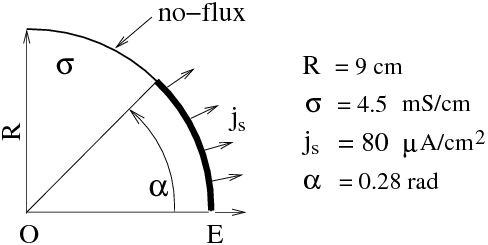
\includegraphics[scale=1]{quadrant.png}
    \caption{Volume conductor model quadrant}
\end{center}
\end{figure}

\begin{figure}[H]
    \begin{center}
        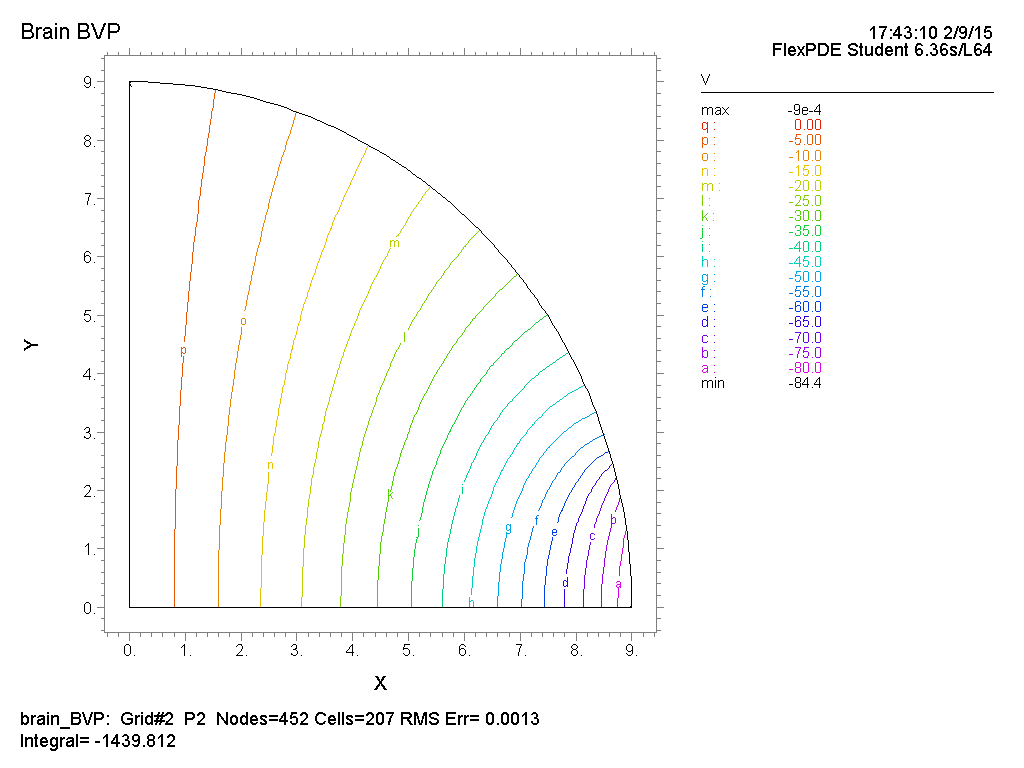
\includegraphics[scale=0.5]{contour_001.png}
        \caption{Contour plot on the quadrant of the volume conductor from flexPDE}
    \end{center}
\end{figure}

\begin{figure}[H]
    \begin{center}
        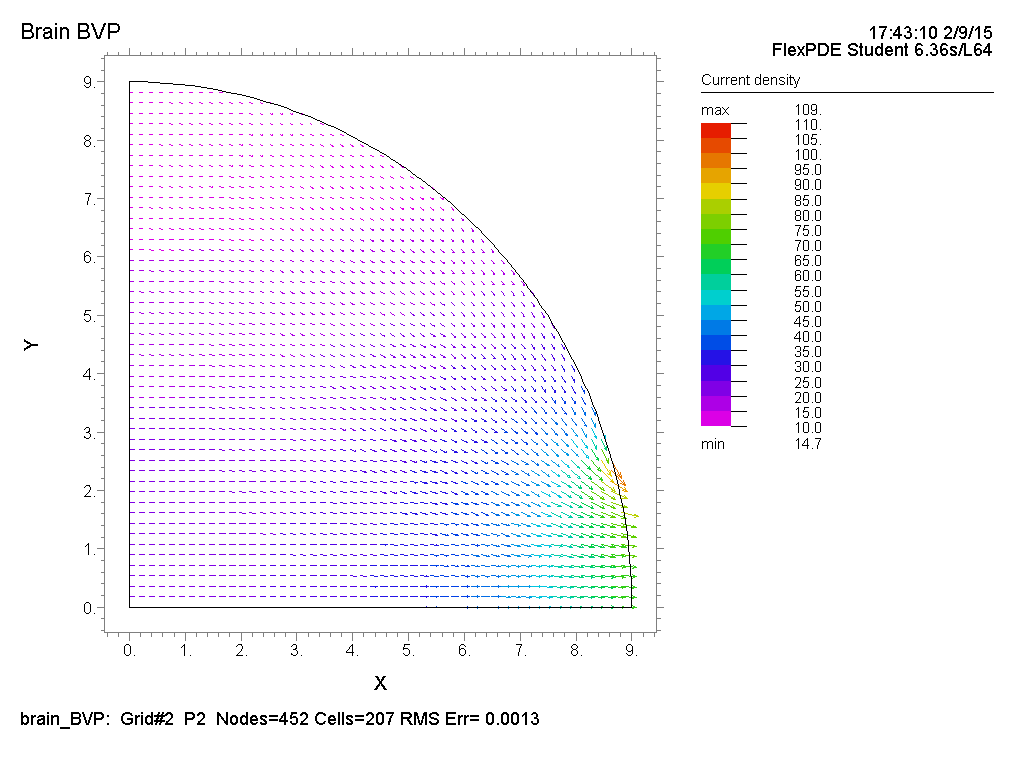
\includegraphics[scale=0.5]{J_vec_001.png}
        \caption{Vector plot of the current density. This is done by plotting $(-\sigma*\nabla V)$}
    \end{center}
\end{figure}

\section{Question 3 \& 4}
The flexPDE plots vs. the analytical plots of the potential, electric field magnitude, and current density are shown below. The flexPDE plots are shown in RED.

\begin{figure}[H]
    \begin{center}
        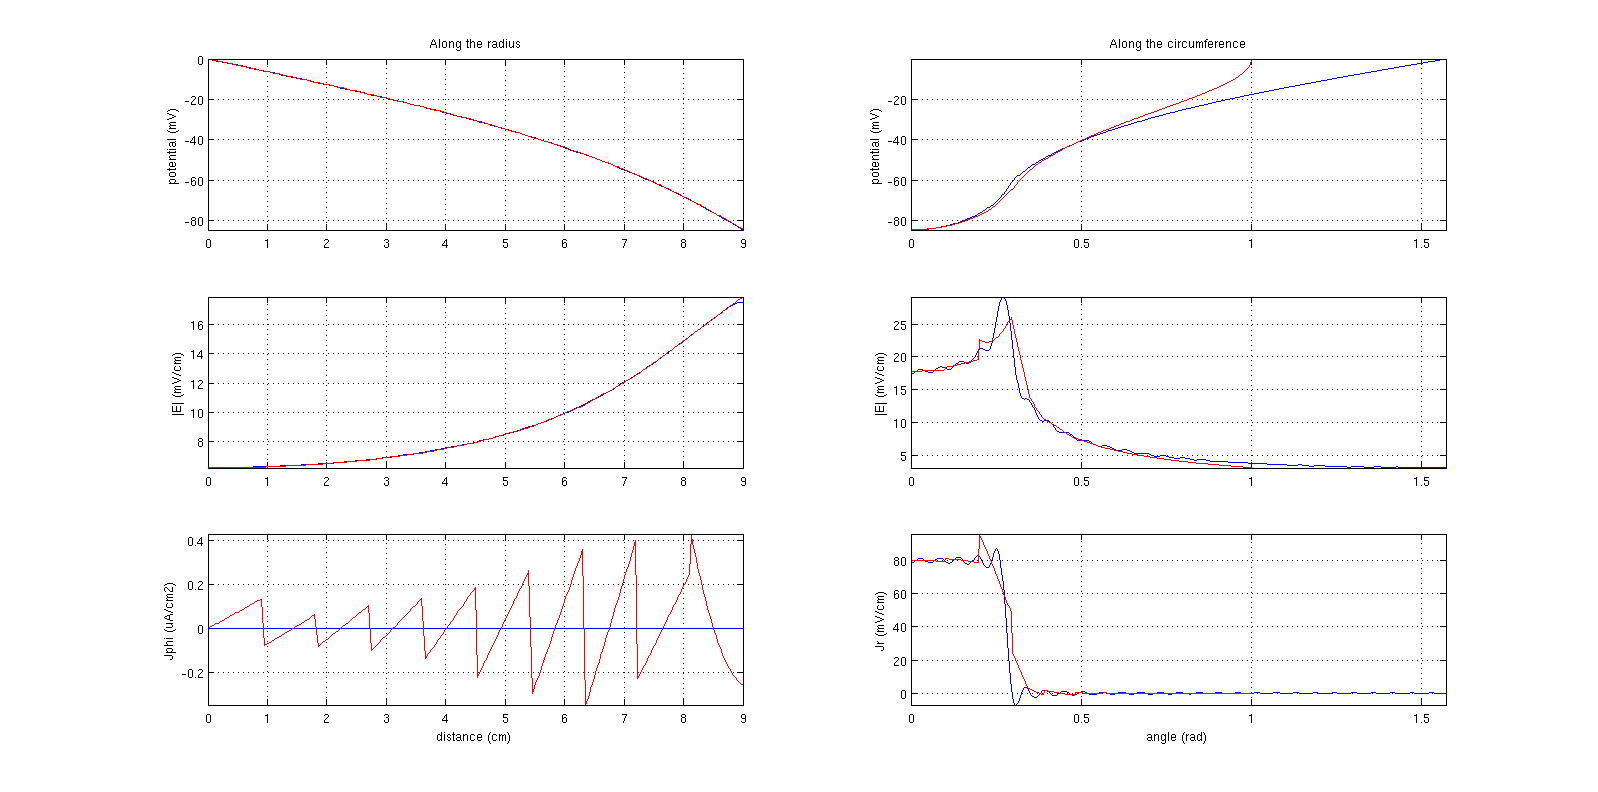
\includegraphics[scale=0.35]{results.png}
        \caption{From left to right, then top to bottom: 1) potential along the path O-E; 2) potential along the circumference; 3) electric field magnitude along the path O-E; 4) electric field magnitude along the circumference; 5) angular component of current density along the path O-E; 6) normal component of current density along the circumference. Blue curves are analytical results. Red curves are flexPDE results.}
    \end{center}
\end{figure}

\section{Question 5}
In the electric field magnitude and current density plots generated by flexPDE, there are many sharp, jagged edges. This suggests that flexPDE uses a linear shape function, which means the mesh points are connected with lines rather than higher order, more smooth polynomial functions.

\section{Question 6}
Comparing the numerical vs. analytical results, we can confirm that the flexPDE yields results with the correct shape and order of magnitude. The numerical results are within $10\%$ of the analytical one. This accuracy can likely be improved with finer mesh grid and higher node counts.

The analytical solution satisfies the boundary conditions better. This is especially obvious in the plot for angular component of current density along the x-axis, where the numerical results demonstrates many zig-zags rather than a flat line at 0. However, this is expected since the anlytical solution must satisfy the boundary conditions perfectly by construction.

\end{document}

